% !TEX root = ../main.tex
%
\section{Introduction}
\label{sec:introduction}

Research on conversational moderation/facilitation techniques is crucial for adapting to ever-changing and demanding online environments. Relevant work traditionally focused on isolating and removing toxic and inappropriate content (``content moderation'') --- \citet{seering_self_moderation, cresci_pesonalized_interventions}, whereas the current social media environment demands platforms to adequately discuss and explain their actions (``conversational moderation'' or ``facilitation'' --- \citet{argyle2023, korre2025evaluation, falk-etal-2021-predicting}); thus preventing problematic user behavior before it surfaces \cite{cho-etal-2024-language, seering_self_moderation, cresci_pesonalized_interventions, make_reddit_great}, supporting community deliberation and group decision-making \cite{kim_et_al_chatbot, seering_self_moderation}.

\begin{figure}[t]
	\centering
	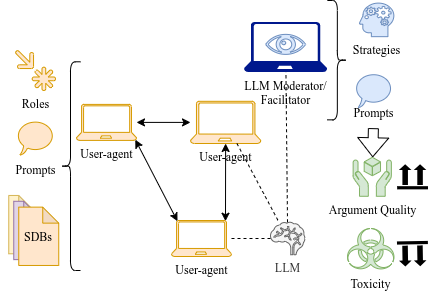
\includegraphics[width=\columnwidth]{research_goal.png}
	\caption{\ac{LLM} user-agents with distinct \acp{SDB} participate in a discussion, while the \ac{LLM} moderator monitors and attempts to improve the quality of the discussion. We need to design prompts and configurations for both types of \ac{LLM} agents.}
	\label{fig::goals}
\end{figure}

A major challenge in connecting facilitation research to real-world needs is the substantial costs required both in researching and moderating discussions, due to human participation \cite{rossi_2024}. This is usually overcome by volunteer users \cite{Matias2019TheCL, schaffner_community_guidelines}, or conventional content moderation using traditional \ac{ML} models, which are not enough in practice \cite{horta_automated_moderation, schaffner_community_guidelines}. \acfp{LLM} have been hypothesized to be capable of facilitation tasks, which often require actively participating in the discussions, instead of passively flagging or removing content \cite{small-polis-llm, korre2025evaluation}. 

While studies exist for simulating user interactions in social media \cite{park_simulacra, mou_2024, tornberg_2023, y_social, balog_2024}, and for using \ac{LLM} facilitators \cite{kim_et_al_chatbot, cho-etal-2024-language}, none so far have combined the two approaches. We posit that synthetic simulations can be a cheap and fast way to develop and test preliminary experiments with \ac{LLM} facilitators, initial versions of which may be unstable or unpredictable \cite{atil_2025, rossi_2024}, before testing them with human participants. Our work thus asks the following two questions: (1) Can we produce high-quality synthetic discussions, involving alternative facilitation strategies, by crafting an appropriate environment for simulations? (2) Are facilitation strategies proposed in modern Social Science research able to help \ac{LLM} facilitators?

We propose a simple and generalizable methodology which enables fast and inexpensive model “debugging” and parameter testing (e.g., discarding sub-optimal  prompts for the \ac{LLM} facilitator) without human involvement (Fig.~\ref{fig::goals}) (\S\ref{sec:methodology}). An ablation study demonstrates that each component of our methodology substantially contributes to generating high-quality data (\S\ref{ssec:results:ablation}). 

Through this methodology, we examine  four \ac{LLM} facilitation strategies based on current Social Science facilitation research and compare them with two common facilitation setups (no facilitator, \acp{LLM} with simplistic prompts) (\S\ref{sec:experimental}). We find that: (1) the presence of \ac{LLM} facilitators has a positive and statistically significant influence on the quality of synthetic discussions, (2) facilitation strategies inspired by Social Science research often do not manage to outperform simpler strategies (\S\ref{ssec:results:main}).

Finally, we release \syndisco, an open-source Python framework which implements our methodology at-scale, alongside \vmd\datasetlink a large, publicly available dataset comprising automatically evaluated synthetic discussions (\S\ref{sec:data-soft}). Our dataset can then be used  for \ac{LLM} facilitator finetuning \cite{ulmer2024}, as well as for observing the behavior of out-of-the-box \acp{LLM} in the task. We use open-source \acp{LLM} and include all relevant configurations in order to make our study as reproducible as possible (see \S\ref{ssec:appendix:annotation}, \S\ref{ssec:appendix:prompts}).